\subsubsection{Impact of Text Conditioning Schemas}
\label{sec:text_conditioning_ablation}

We ablate various schemas for conditioning the frozen text embeddings in the base $64\times64$ text-to-image diffusion model. Fig. \ref{fig:text_cond_comparison} compares the CLIP-FID pareto curves for mean pooling, attention pooling, and cross attention. We find using any pooled embedding configuration (mean or attention pooling) performs noticeably worse compared to attending over the sequence of contextual embeddings in the attention layers. We implement the cross attention by concatenating the text embedding sequence to the key-value pairs of each self-attention layer in the base $64\times64$ and $64\times64 \rightarrow 256\times256$ models. %
For our $256\times256 \rightarrow 1024\times1024$ model, since we have no self-attention layers, we simply added explicit cross-attention layers to attend over the text embeddings. We found this to improve both fidelity and image-text alignment with minimal computational costs. 



\begin{figure}[t]
    \centering
    \begin{subfigure}[t]{0.49\textwidth}
    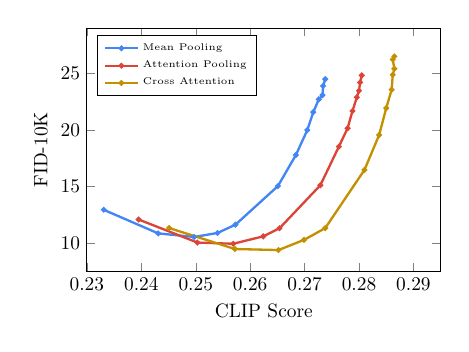
\begin{tikzpicture}[scale=0.7]

\definecolor{google_blue}{RGB}{66,133,244}
\definecolor{google_red}{RGB}{219,68,55}
\definecolor{google_yellow}{RGB}{194,144,0}
\definecolor{google_green}{RGB}{15,157,88}


\begin{axis}[width=8cm, height=6cm,
  xlabel=CLIP Score,
  ylabel=FID-10K,
  legend columns=1,
  legend pos=north west,
  legend cell align=left,
  legend style={font=\tiny},
  xmin=0.23,
  ymin=7.5,
  ymax=29,
  xmax=0.295,
  every axis plot/.append style={very thick}
]
\addplot +[mark=*, solid, google_blue, mark options={scale=0.4}] coordinates {(0.2331, 12.9559)(0.2431, 10.874)(0.2497, 10.556)(0.254, 10.9103)(0.2573, 11.6425)(0.2651, 15.0507)(0.2684, 17.7926)(0.2705, 19.9939)(0.2716, 21.5785)(0.2726, 22.7001)(0.2733, 23.0793)(0.2734, 23.8903)(0.2738, 24.4911)};

\addplot +[mark=*, solid, google_red, mark options={scale=0.4}] coordinates {(0.2395, 12.0989)(0.2503, 10.0628)(0.2569, 9.9583)(0.2624, 10.6117)(0.2654, 11.3276)(0.2729, 15.1281)(0.2763, 18.5341)(0.2779, 20.1554)(0.2788, 21.6792)(0.2796, 22.8844)(0.28, 23.4682)(0.2802, 24.2021)(0.2805, 24.8261)};

\addplot +[mark=*, solid, google_yellow, mark options={scale=0.4}] coordinates {(0.2451, 11.3483)(0.2572, 9.4933)(0.2652, 9.4017)(0.2699, 10.2998)(0.2738, 11.3422)(0.281, 16.4762)(0.2837, 19.563)(0.285, 21.9303)(0.286, 23.5618)(0.2862, 24.8776)(0.2865, 25.403)(0.2862, 26.2234)(0.2865, 26.5037)};

\legend{Mean Pooling, Attention Pooling, Cross Attention}
\end{axis}
\end{tikzpicture}
    \caption{Comparison between different text encoders.}
     \label{fig:text_cond_comparison}
    \end{subfigure}
    \begin{subfigure}[t]{0.49\textwidth}
     \centering
     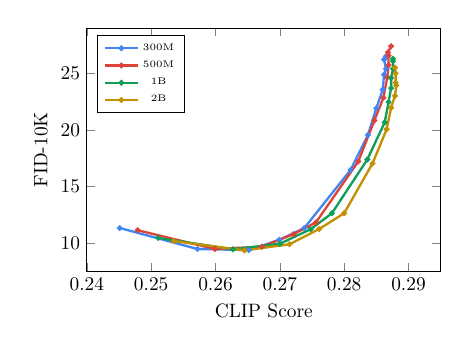
\begin{tikzpicture}[scale=0.7]

\definecolor{google_blue}{RGB}{66,133,244}
\definecolor{google_red}{RGB}{219,68,55}
\definecolor{google_yellow}{RGB}{194,144,0}
\definecolor{google_green}{RGB}{15,157,88}


\begin{axis}[width=8cm, height=6cm,
  xlabel=CLIP Score,
  ylabel=FID-10K,
  legend columns=1,
  legend pos=north west,
  legend style={font=\tiny},
  xmin=0.24,
  ymin=7.5,
  ymax=29,
  xmax=0.295,
  every axis plot/.append style={very thick}
]
\addplot +[mark=*, solid, google_blue, mark options={scale=0.4}] coordinates {(0.2451, 11.3483)(0.2572, 9.4933)(0.2652, 9.4017)(0.2699, 10.2998)(0.2738, 11.3422)(0.281, 16.4762)(0.2837, 19.563)(0.285, 21.9303)(0.286, 23.5618)(0.2862, 24.8776)(0.2865, 25.403)(0.2862, 26.2234)(0.2865, 26.5037)};
\addplot +[mark=*, solid, google_red, mark options={scale=0.4}] coordinates {(0.2479, 11.1512)(0.2599, 9.4931)(0.2672, 9.7014)(0.2721, 10.7983)(0.2756, 11.8326)(0.2822, 17.2267)(0.2847, 20.8375)(0.2861, 22.856)(0.2867, 24.6328)(0.2869, 25.723)(0.2869, 26.5768)(0.2868, 26.8506)(0.2873, 27.3912)};
\addplot +[mark=*, solid, google_green, mark options={scale=0.4}] coordinates {(0.2511, 10.4663)(0.2627, 9.4659)(0.27, 9.9582)(0.2748, 11.2437)(0.2781, 12.6562)(0.2836, 17.3972)(0.2863, 20.673)(0.2869, 22.4689)(0.2873, 23.7)(0.2873, 24.6056)(0.2876, 25.4052)(0.2876, 26.0697)(0.2876, 26.2802)};
\addplot +[mark=*, solid, google_yellow, mark options={scale=0.4}] coordinates {(0.2535, 10.1896)(0.2645, 9.3721)(0.2715, 9.9115)(0.2761, 11.2531)(0.28, 12.6531)(0.2844, 17.0384)(0.2866, 20.061)(0.2873, 21.9676)(0.2879, 23.0162)(0.2881, 23.936)(0.288, 24.1819)(0.288, 25)(0.2879, 25.5056)};

\legend{300M, 500M, 1B, 2B}
\end{axis}
\end{tikzpicture}
      \caption{Comparison between different model sizes.}
      \label{fig:model_size_comparison}
    \end{subfigure}
    \caption{CLIP vs FID-10K pareto curves for different ablation studies for the base $64\times64$ model. For each study, we sweep over guidance values of $[1, 1.25, 1.5, 1.75, 2, 3, 4, 5, 6, 7, 8, 9, 10]$}
\end{figure}
